\documentclass[a4paper, 12pt]{article}
%############################ Language
%% Language and font encodings
\usepackage[english]{babel}
\usepackage[utf8]{inputenc}

\usepackage{booktabs}
\usepackage{tabu}
\usepackage[T1]{fontenc}
%########################### Paper
%% Sets page size and margins
\usepackage[a4paper,top=3cm,bottom=3cm,left=3cm,right=3cm,marginparwidth=1.75cm]{geometry}
\setlength {\marginparwidth }{2cm}

%% Useful packages
\usepackage{amsmath}
\usepackage{mathtools}
\usepackage{graphicx}
\usepackage{etoolbox} % For modifying thebibliography
\usepackage[colorinlistoftodos]{todonotes}
\usepackage[colorlinks=true, allcolors=blue]{hyperref}

\usepackage{parskip} % exchanges indentation for spacing between paragraphs.

%############################ Header 
\usepackage{fancyhdr} 
\usepackage{lastpage} % \lastpage
\pagestyle{fancy}
\fancyhead{}
\fancyfoot{}
\setlength{\headheight}{15pt}
\fancyhead[L]{V. Ballester and J. Nägerl} %welcher Versuch 
\fancyhead[R]{\itshape\nouppercase{\leftmark}}
\fancyfoot[C]{Page \thepage\ }
\pagestyle{fancy}

%############################ Graphics
\usepackage{caption}
\captionsetup{font=scriptsize}
\usepackage{wrapfig} 
%############################ References 
% Modify the font size of the bibliography
\patchcmd{\thebibliography}{\fontsize{1}{1}}{\fontsize{1}{1}}{}{}
\usepackage{bibliography}


%%% ad subsubsection to 

%############################ CODE
\usepackage{listings}
\usepackage{graphicx}
\usepackage{float}
\usepackage{xcolor}
\usepackage{math}

\definecolor{codegreen}{rgb}{0,0.6,0}
\definecolor{codegray}{rgb}{0.5,0.5,0.5}
\definecolor{codepurple}{rgb}{0.58,0,0.82}
\definecolor{backcolour}{rgb}{0.95,0.95,0.92}

\lstdefinestyle{mystyle}{
    backgroundcolor=\color{backcolour},
    commentstyle=\color{codegreen},
    keywordstyle=\color{magenta},
    numberstyle=\tiny\color{codegray},
    stringstyle=\color{codepurple},
    basicstyle=\ttfamily\scriptsize,
    breakatwhitespace=false,
    breaklines=true,
    captionpos=b,
    keepspaces=true,
    numbers=left,
    numbersep=5pt,
    showspaces=false,
    showstringspaces=false,
    showtabs=false,
    tabsize=2
}

\lstset{style=mystyle}

%############################ Title page
%################################################
%############################ Document
%################################################
\renewcommand\title{Numerical simulation of von Kármán vortex streets}
\renewcommand\author{Víctor Ballester\\Jona Nägerl}
\renewcommand\date{March 05, 2023}
\newcommand\supervisor{Guillaume Legendre\\Gabriel Turinici}
\newcommand\department{MIDO department}
\newcommand\degree{M2 Applied and Theoretical Mathematics}


\begin{document}
\begin{titlepage}
  \begin{center}
    \begin{figure}[H]
      \begin{center}
        
\includegraphics[width=6cm]{0_graphics/dauphine-psl.pdf}
      \end{center}
    \end{figure}
    \vspace*{1.5cm}
    \textsc{\Large Numerical methods for deterministic and stochastic problems }\\[0.75cm]
    \rule{150mm}{0.1mm}\\[0.4cm]
    {\huge \bfseries \title\par}
    \vspace{0.4cm} % Thesis title
    \rule{150mm}{0.1mm} \\[1.5cm] % Horizontal line
    \begin{minipage}[ht]{0.4\textwidth}
      \begin{flushleft} \large
        \emph{Authors:}\\[0.2cm]
        \author % Author name - remove the \href bracket to remove the link
      \end{flushleft}
    \end{minipage}
    \begin{minipage}[ht]{0.4\textwidth}
      \begin{flushright} \large
        \emph{Supervisors:} \\[0.2cm]
        \supervisor % Supervisor name - remove the \href bracket to remove the link  
      \end{flushright}
    \end{minipage}\\[3cm]
    \vfill
    {\large
      \degree\\[0.2cm]
      \department\\[0.2cm]
    }
    % \vfill
    \rule{80mm}{0.1mm}\\[0.5cm]
    {\large \date}\\[0.2cm]
    \vfill
  \end{center}
  \newpage
\end{titlepage}
% \begin{center}  
% \LARGE
% Report Numerical Methods  
% \vspace{0.5cm} 
% \rule{\textwidth}{1.5pt}
% \LARGE
% \textbf{\mytitle}
% \rule{\textwidth}{1.5pt}
% \vspace{3cm}    
% \large
% \\

% \vfill
% \Large
% \textbf{\myname}
% \vfill
% \large
% Paris, February 27\textsuperscript{th}, 2024     
% \vfill
% 
\includegraphics[width = 0.4\textwidth]{0_graphics/dauphine-psl_2.png}
% \vfill
% \normalsize


% \end{center}
% \end{titlepage}

% change color of the links (linkcolor)
\hypersetup{linkcolor=black}
\tableofcontents
% change it back
\hypersetup{linkcolor=red!60!black}
% ###################################################################
% ######## CONTENT
% ###################################################################
\newpage
\section{Introduction} \label{sec: intro}
In the study of fluid dynamic systems, the \textit{von Kármán vortex street} phenomenon stands a classical example of pattern formation in flows behind bodies. The pattern is characterized by alternating vortices, and it is not just an example of the complexity of fluid dynamics, but also of great importance in various research fields influencing the design of objects in fluid or aerodynamic systems. For example, the performance of a wing heavily depends on the specific flow, and therefore emergence of vortices can have an impact on the efficiency of the plane and its flight capabilities in various situations. The potential optimization of shape and coatings to achieve desired flight performances led alone in the field of aircraft engineering to a multitude of studies and research activities. Another very interesting occurrence of the phenomenon is shown in \cref{fig: example vortices}, where the interplay of a mountain and wind leads to pattern formation in the clouds and forms alternating vortices. 

\begin{figure}[!htb]
        \centering
        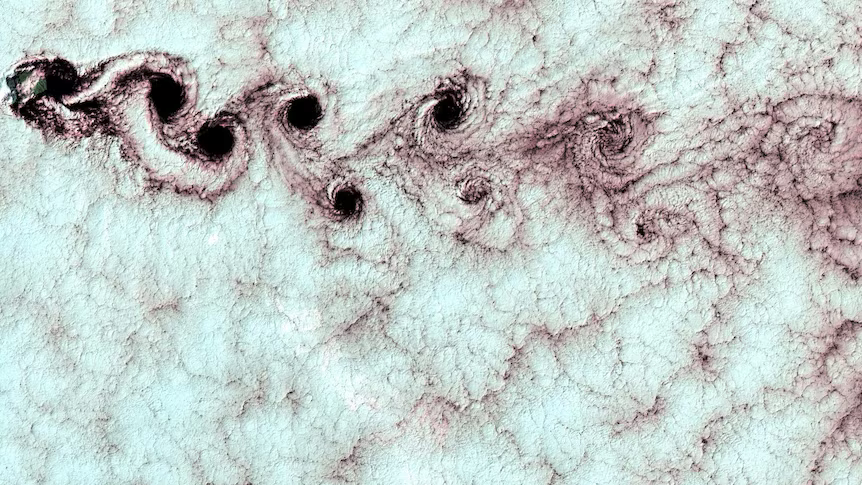
\includegraphics[width=0.6\linewidth]{0_graphics/example_atmos.png}
        \caption{View of a von Kármán vortex street in the atmosphere, showcasing the pattern of swirling vortices caused by airflow around a mountain \cite{wiki}.}
        \label{fig: example vortices}
\end{figure}

This project aims to numerically simulate this phenomenon in a two-dimensional flow field. By leveraging the \textit{Chorin projection method} to decouple the velocity and pressure fields and using a \textit{Semi-Langrangian} solver for the advective term in the underlying equations, we aim to simplify the computational complexity inherent in fluid dynamics problems and to ensure stability and accuracy in the representation of vortex shedding and evolution over time.
Therefore, the plan for the following report is as follows.

First, we introduce the underlying equations as well as the boundary conditions in \cref{sec: posingProblem} that we deal with, and present and motivate the solver in \cref{sec: diffScheme}. In \cref{sec: results}, we numerically simulate the system and investigate the flow patterns for various setups and different shapes.
% \newpage

\section{Methods}\label{sec: methods}
%Here a lot is missing but for first start I have copied the graphics which content should be included here REFERENCE_numerical. Page 271 main reference \cite{numeric_method_book}
\subsection{Posing the problem} \label{sec: posingProblem}
To simplify our approach we look at a two-dimensional incompressible fluid. In this section we want to pose the problem by introducing the underlying mathematical equations and discuss the boundary conditions.

\subsubsection*{Underlying equations}
In our approach we simplify the problem to a two-dimensional incompressible viscous fluid in a rectangular domain box flowing from one side of the box to the other, encountering an obstacle in its path. The motion of the fluid is described by the \textit{incompressible Navier-Stokes equation}

\begin{align}
  \rho \left( \frac{\partial \textbf{u}}{\partial t}  + \textbf{u} \cdot \nabla \textbf{u} \right)- \mu \Delta \textbf{u}+ \nabla p =0 \label{eq: incompressNS} \\
  \nabla\cdot \textbf{u} = 0 \notag
\end{align}

where $\rho$ is the mass density (assumed constant), $\textbf{u} = (u,v)$ is the fluid velocity with horizontal component $u$ and vertical component $v$, $\mu$ is the dynamic viscosity of the fluid and $p$ is the pressure. The first equation encapsulates the momentum balance within the fluid, incorporating the effects of advection ($\textbf{u} \cdot \nabla \textbf{u}$, velocity interaction and movement), diffusion ($\mu \Delta \textbf{u}$, velocity spreading due to viscosity), and the pressure gradient's influence on the fluid motion ($\nabla p$), whereas the second equation, often termed the \textit{continuity equation}, asserts the incompressibility of the fluid by ensuring the volume conservation within the flow. The equations can be adimensionalized with the following change of variables

\begin{align}
  \Tilde{\textbf{u}} = \frac{\textbf{u}}{U}, \quad \Tilde{p} = \frac{p}{\rho U^2}, \quad \Tilde{\textbf{x}} = \frac{\textbf{x}}{L}, \quad \Tilde{t} = \frac{U}{L}t
\end{align}

where the characteristic velocity $U$ and characteristic length $L$ are used. These quantities represent the typical velocity of the fluid and typical lengthscale. In practice, they are taken to be the inflow velocity and the length of the obstacle in the transverse direction to the flow, respectively. Applying these change of variables to \cref{eq: incompressNS}, we get (dropping the tilde for readability):

\begin{align}
  \frac{\partial \textbf{u}}{\partial t} + \textbf{u} \cdot \nabla \textbf{u} - \frac{1}{\text{Re}} \Delta \textbf{u} + \nabla p = 0 \label{eq:Ns_normalized} \\
  \nabla\cdot\vf{u} = 0 \notag
\end{align}

where the Reynolds number $\Rey := \frac{\rho U L}{\mu}$ is a dimensionless parameter that measures the ratio between the inertia of the flow and the viscosity of it.

\subsubsection*{Boundary conditions}
%The body is first time mentionend here but will be explained later
The domain $\Omega$ is the rectangular box without the obstacle. We call the horizontal direction $x$-direction and the vertical direction $y$-direction. In our study, on the left side a laminar flow is coming into the domain. At the beginning the fluid inside the box is at rest and pressure is null within the domain. At the horizontal walls a slip condition is imposed and a free flow on the right side is assumed. Therefore we obtain as boundary conditions for the walls:

\begin{itemize}
  \item At time $t=0$, the fluid is at rest, and both velocity and pressure are zero.
  \item On the left side, the flow is incoming with a velocity equal to $U \mathbf{e}_x$, and the pressure satisfies the conditions $\frac{\partial p}{\partial x} = 0$.
  \item On the right side of the domain, the flow is free so that $\frac{\partial u}{\partial x} = \frac{\partial v}{\partial x} = 0$ and $p = 0$.
  \item On the horizontal sides, the walls are impenetrable, so that $v = 0$. A slip condition is imposed so that $\frac{\partial u}{\partial y} = 0$ and $\frac{\partial p}{\partial y} = 0$.
\end{itemize}

In order to accurately implement these boundary conditions, we make use of the \textit{ghost cell} method. This technique involves the addition of a layer of cells outside the domain (see \cref{fig: ghostCells}), called \textit{ghost cells}. These cells are used to approximate at second order the values of the velocity and pressure at the boundary for both Dirichlet and Neumann boundary conditions.

\begin{figure}[h]
  \centering
  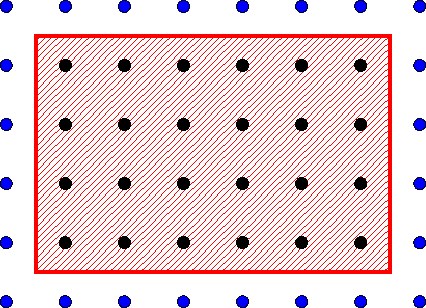
\includegraphics[width=0.5\textwidth]{0_graphics/methods/grid.pdf}
  \caption{The ghost cell method. The domain $\Omega$ is represented in red and the dots represent the grid cells, the black ones being the inner cells and the blue ones, the ghost cells.}
  \label{fig: ghostCells}
\end{figure}

As an example, if $u_{0,j}$ denotes the horizontal component of $\vf{u}$ at the left boundary and height $j$ (counting from 0), then it is approximated by $2U-u_{1,j}$, where $u_{1,j}$ is the horizontal component of $\vf{u}$ at the first cell inside the domain and the same height $j$. A straightforward Taylor expansion around the boundary point (say $u_{1/2,j}$) shows us that indeed this approximation is of second order. Similarly, we obtain values for $v_{0,j}$ and $p_{0,j}$ as

$$
  v_{0,j} = -v_{1,j}, \quad p_{0,j} = p_{1,j}
$$

The other boundaries are treated in the same way, but exchanging the role between $i$ and $j$ and taking into account the different boundary conditions. It should be noted that when computing discrete derivatives, which involve the use of neighbouring cells, the computations are carried out only on the inner cells, which in turn use ghost cells. But the derivatives themselves at ghost cells are never computed.

We discuss now the treatment of the boundary conditions on the object. In general dealing with the object is not an easy task. For simplicity, we model the presence of a solid body within a fluid by enforcing the fluid velocity to be zero inside the object, which correspond to imposing a no-slip condition at the boundary. We can think of it as a direct forcing method, which is a common approach in the literature, and it is based on the idea of adding a forcing term to the Navier-Stokes equations to account for the presence of the object (see \cite{forcing} for more details).
It is very worth-mentioning that the way we integrate the body has an influence on the flow. Especially to study the impacts of coatings or surface structure, our method, is not capable of including these effects, but in our approach we only want to observe the effect, and therefore prioritize simplicity for understanding over complexity for small details in the effect. If the reader is interested in delving deeper into the fluid-structure interactions, including the effects of surface modifications, we recommend consulting works in the field, such as those by Peskin \cite{Peskin1977ImmersedBM} or Schlichting and Gersten \cite{Schlichting2000BoundaryLayerT}.

\subsection{Difference Scheme} \label{sec: diffScheme}
In this section we discuss our numerical solver to integrate \cref{eq:Ns_normalized} together with the boundary conditions presented in above section. To simplify the equations, we use \textit{Chorin's projection method}. It was originally introduced by Alexandre Chorin in 1967 \cite{Chorin1967NumericalNS} as an efficient means of solving the incompressible Navier-Stokes equations.

The idea of the method is to first predict the velocities for the next time step by solving the advection and the diffusion term. With the intermediate velocity field we solve the Poisson equation with a finite difference method (described below). Finally, the \textit{projection step} is preformed, and the velocity field is updated with the new pressure field.

This method is based on the Helmholtz-Hodge decomposition of a vector field $\vf{F}$, which states that any vector field can be decomposed into a sum of a solenoidal (divergence-free) and an irrotational (curl-free) part. In our of fluid dynamics, this means that the velocity field $\vf{u}^*$ can be decomposed into a sum of a solenoidal part $\vf{u}^{n+1}$ and an irrotational part $\nabla p^{n+1}$, where $p^{n+1}$ is the pressure field at time $t^{n+1}$. The projection step is then used to enforce the incompressibility of the velocity field, and to update the velocity field with the new pressure field. 

To ensure that the boundary conditions are met, we impose the conditions for the velocity right before solving the Poisson equation and at the end of each iteration. The boundary conditions for the pressure are imposed after solving the Poisson equation and before correcting the velocities in the projection step.

Next, we provide a summary of the steps in our method. Assuming we know the velocity field at time $t^n$, $\vf{u}^n$, we want to compute the velocity field at time $t^{n+1}$, $\vf{u}^{n+1}$.
\begin{enumerate}
  \item Solve for $\vf{u}^a$ in $\displaystyle  \frac{\vf{u}^a-\vf{u}^n}{\Delta t} + \vf{u}^n \cdot \nabla \vf{u}^n = 0$ using a semi-Lagrangian method.
  \item Solve for $\vf{u}^*$ in $\displaystyle  \frac{\vf{u}^* - \vf{u}^a}{\Delta t} = \frac{1}{\Rey} \laplacian \vf{u}^n$.
  \item Set the boundary conditions for the intermediate velocity field $\vf{u}^*$ and impose the velocity field $\vf{u}^*$ inside the object to be zero (forcing term).
  \item Solve the Poisson equation for the pressure, $\displaystyle \laplacian p^{n+1} = \frac{1}{\Delta t}\nabla \cdot \vf{u}^*$.
  \item Set the boundary conditions for the pressure $p^{n+1}$.
  \item Project the pressure to the intermediate velocity to obtain the new velocity at time $t^{n+1}$, $\displaystyle \vf{u}^{n+1} = \vf{u}^* - \Delta t\nabla p^{n+1}$.
  \item Set the boundary conditions for the velocity field $\vf{u}^{n+1}$.
\end{enumerate}
From these equations, one can easily check that we have:
\begin{align*}
  \frac{\vf{u}^{n+1}-\vf{u}^n}{\Delta t} + \vf{u}^n \cdot \nabla \vf{u}^n - \frac{1}{\Rey} \laplacian \vf{u}^n + \nabla p^{n+1} & = 0 \\
  \nabla \cdot \vf{u}^{n+1}                                                                                                   & = 0
\end{align*}

In the following sections we deepen in how do we compute each of the above steps in our method.

\subsubsection*{Semi-Lagrangian method}
% What is a Semi-Langrangian method
The Semi-Lagrangian (SL) method represents a powerful approach to solving fluid dynamics problems, particularly in the context of advection. Unlike Eulerian methods, which compute changes at fixed points in space, the SL method tracks the motion of fluid parcels. SL methods slightly differ from Lagrangian methods, as the word suggests. The second ones are rarely used in numerical methods because the particle trajectories become chaotic and wildly mixed in a short period of time. However, SL algorithms avoid this problem by \textit{reinitializing} the Lagrangian coordinate system after each time step \cite{Boyd2001ChebyshevFourier}. There are several ways to implement a SL method, and we describe here the one we used in our method. Our goal in this subsection is on solving:

\begin{equation*}
  \frac{\mathrm{D}\vf{u}}{\mathrm{D}t} = \pdv{\vf{u}}{t} + \vf{u} \cdot \nabla \vf{u} = 0
\end{equation*}

The idea is to somehow discretize the material derivative. To do that, if we call $\vf{u}^n$ the current velocity field and $\vf{u}^a$ the velocity field after the advection step, we can write a difference formula as:

\begin{equation*}
  \frac{\vf{u}^a- \vf{u}^n}{\Delta t} + \vf{u}^n \cdot \nabla \vf{u}^n = 0
\end{equation*}

The following discretization for the material derivative is used:

\begin{equation*}
  \frac{\vf{u}(\vf{x}_{i,j},t^{n+1})  - \vf{u}(\vf{x}_{i,j} - \vf{u}(\vf{x}_{i,j},t^n)\Delta t,t^n)}{\Delta t} = 0
\end{equation*}

Here we are approximating the solution along a characteristic line, which generally differs from the actual characteristic associated to the solution at that point, with a constant velocity of $\vf{u}(\vf{x}_{i,j},t^n)$ at each grid point $\vf{x}_{i,j}$.
The reader may rapidly notice that the point $\vf{x}_{i,j} - \vf{u}(\vf{x}_{i,j},t^n)\Delta t$ is not in general in the grid, and thus, we don't have the respective value of the velocity field. To solve this problem, we make use of bilinear interpolation between the four (in 2D) surrounding grid points to the point $\vf{x}_{i,j} - \vf{u}(\vf{x}_{i,j},t^n)\Delta t$. This gives us an approximation of the velocity field at the point $\vf{x}_{i,j} - \vf{u}(\vf{x}_{i,j},t^n)\Delta t$, which in turn provides us with the advected velocity field $\vf{u}^a$.

Furthermore, to improve the accuracy of the method we use the back-and-forth method \cite{backforth}. This method first advects the velocity field using the method described above, and then advects back with opposite velocity $\vf{u}\to -\vf{u}$. With this, we can have an estimate of the error we are comitting when comparing the last result with the initial position. Using this information we can correct the initial velocity field and obtain a more accurate result. The steps are reproduced below. In order to make things more clear, we consider the general case:

\begin{equation*}
  \frac{\mathrm{D}\vf{\psi}}{\mathrm{D}t} = \pdv{\vf{\psi}}{t} + \vf{u} \cdot \nabla \vf{\psi} = 0
\end{equation*}

\begin{enumerate}
  \item Advect the field $\vf\psi^n$ with velocity $\vf{u}$ to obtain $\tilde{\vf{\psi}}^a$.
  \item Advect the field $\vf{\tilde{\psi}}^a$ with velocity $-\vf{u}$ to obtain $\vf{\bar{\psi}}^a$.
  \item Advect the field $\vf{\psi}^n + \frac{1}{2} (\vf{{\psi}}^n - \vf{\bar{\psi}}^a)$ with velocity $\vf{u}$ to obtain $\vf{\psi}^a$.
\end{enumerate}

In our case, the field $\vf\psi$ exactly corresponds to the same velocity field $\vf{u}$. This approach has been proved to be stable and improving considerably the accuracy of the method \cite{backforth}. 

Last but not least, as in all hyperbolic equations, the Courant-Friedrichs-Lewy (CFL) condition must be satisfied. This condition states that the time step $\Delta t$ must be chosen such that the real solution propagates at most at the same speed as the numerical solution. Thus, since we are using an explicit scheme we must impose a CFL of

$$|u|_{\text{max}} \frac{\Delta t}{\Delta x} +|v|_{\text{max}} \frac{\Delta t}{\Delta y}\leq 1$$

\subsubsection*{Diffusion term}
As a second step we add diffusion using a second order central differences. The diffusion term is given by:

\begin{equation*}
  \frac{\vf{u}^* - \vf{u}^a}{\Delta t} = \frac{1}{\Rey} \laplacian \vf{u}^n
\end{equation*}

Once discretized we get for each $i$, $j$ in the grid:

\begin{equation*}
  \vf{u}^*_{i,j} = \vf{u}^a_{i,j} + \frac{\Delta t}{\Rey}\left( \frac{\vf{u}^n_{i+1,j} - 2\vf{u}^n_{i,j} + \vf{u}^n_{i-1,j}}{{(\Delta x)}^2} + \frac{\vf{u}^n_{i,j+1} - 2\vf{u}^n_{i,j} + \vf{u}^n_{i,j-1}}{{(\Delta y)}^2}\right)
\end{equation*}

We write concisely the discretization in vector form, but in practice we do it for each component of the velocity field separately.

\subsubsection*{Solving for the Poisson equation}\label{sec: solvingPoisson}
There are several efficient ways to compute the solution of the general Poisson equation $\Delta p = f$. In our case, we have to equip this equation with the boundary conditions $\partial_{\vf{n}}p=0$ on the left, top and bottom boundaries, and $p=0$ on the right boundary. We use a finite difference method to solve this equation with a 5-point stencil to approximate the Laplacian operator. The 5-point stencil is given by:

\begin{equation*}
  \laplacian p_{i,j} = \frac{p_{i+1,j} - 2 p_{i,j} + p_{i-1,j}}{{(\Delta x)}^2} + \frac{p_{i,j+1} - 2 p_{i,j} + p_{i,j-1}}{{(\Delta y)}^2}
\end{equation*}

If we set $\vf{p}:=(p_{1,1}, p_{1,2}, \ldots, p_{1,n_y}, p_{2,1}, p_{2,2}, \ldots, p_{2,n_y},\ldots, p_{n_x,1},p_{n_x,2},\ldots p_{n_x,n_y})$, we can write our problem in matrix form as $\vf{A}\vf{p}=\vf{f}$, where $\vf{f}$ contains the discrete values at the grid points of the right-hand side of the Poisson equation in the same order as $\vf{p}$, and $\vf{A}$ is a matrix that contains the coefficients of the discrete Laplacian. To describe how we can build the matrix $\vf{A}$, let $\vf{A}=\vf{X} + \vf{Y}$, where $\vf{X}$ and $\vf{Y}$ denote the matrices that contain the coefficients of the Laplacian operator in the $x$ and $y$ directions, respectively. We can write $\vf{X}$ and $\vf{Y}$ as:

\begin{equation*}
  \vf{X} = \begin{pmatrix}
    -\vf{I}_{n_y} & \vf{I}_{n_y}   & \vf{0}         & \cdots       & \cdots         & \vf{0}         \\
    \vf{I}_{n_y}  & -2\vf{I}_{n_y} & \vf{I}_{n_y}   & \ddots       &                & \vdots         \\
    \vf{0}        & \vf{I}_{n_y}   & -2\vf{I}_{n_y} & \vf{I}_{n_y} & \ddots         & \vdots         \\
    \vdots        & \ddots         & \ddots         & \ddots       & \ddots         & \vf{0}         \\
    \vdots        &                & \ddots         & \vf{I}_{n_y} & -2\vf{I}_{n_y} & \vf{I}_{n_y}  \\
    \vf{0}        & \cdots         & \cdots         & \vf{0}       & \vf{I}_{n_y}   & -3\vf{I}_{n_y} \\
  \end{pmatrix}\quad
  \vf{Y} = \begin{pmatrix}
    \vf{B} & \vf{0} & \cdots & \vf{0} \\
    \vf{0} & \vf{B} & \ddots & \vdots \\
    \vdots & \ddots & \ddots & \vf{0} \\
    \vf{0} & \cdots & \vf{0} & \vf{B} \\
  \end{pmatrix}
\end{equation*}

with

$$
  \vf{B} = \begin{pmatrix}
    -1     & 1      & 0      & \cdots & 0      \\
    1      & -2     & 1      & \ddots & \vdots \\
    0      & \ddots & \ddots & \ddots & 0      \\
    \vdots & \ddots & 1      & -2     & 1      \\
    0      & \cdots & 0      & 1      & -1     \\
  \end{pmatrix}\in\mathcal{M}_{n_y}(\mathbb{R})
$$

Both $\vf{X}$ and $\vf{Y}$ are block matrices, composed of $n_x$ matrices in each row and column of size $n_y\times n_y$ each, which results in a matrix of size $n_xn_y\times n_xn_y$. 
The boundary conditions (using ghost cells) on the pressure are applied at both the first and last block rows of $\vf{X}$ and the first and last rows of $\vf{B}$.

In order to solve the resulting system, we use the Cholesky decomposition, which requires the matrix to be symmetric and positive definite. The matrix $\vf{A}$ is symmetric, but it is not positive definite. In fact, it can be seen that it is negative definite. Thus, in our case, we solve the equivalent system $-\vf{A} \vf{p} = -\vf{f}$.


\subsubsection*{Updating velocities}

As a final step, we compute the gradient of the pressure field and update the velocity field. The gradient of the pressure field is computed using a 2nd order central differences scheme. The update of the velocity field is given by:

\begin{equation*}
  \vf{u}_{i,j}^{n+1} = \vf{u}_{i,j}^* - \Delta t \left(
  \frac{p_{i+1,j}^{n} - p_{i,j}^{n}}{\Delta x}, \frac{p_{i,j+1}^{n} - p_{i,j}^{n}}{\Delta y}
  \right)
\end{equation*}

% \newpage

\section{Results}\label{sec: results}
The method was implemented in C++ using the \texttt{Eigen} library for linear algebra operations \cite{eigen}, particularly for the creation of the sparse matrix $\vf{A}$ described above and the resolution of the resulting linear system using the Cholesky decomposition. We opted not to employ parallelization for the sake of simplicity. However, readers may observe that for achieving more accurate results, such as using a denser grid around the boundary of the object and thereby expanding the size of the discrete domain, parallelization becomes essential\footnote{For further details on the implementation, we shared our code in \href{https://github.com/victorballester7/von-karman}{this} Github repository. There the reader will also find animations of the flow dynamics around different objects to better understand the phenomenon.}

Implementing the numerical scheme outlined in \cref{sec: diffScheme} we have the opportunity to explore the dynamics of fluid flow around various objects. First, we want to illustrate the emergence of the phenomenon before delving in different factors on the flow as differences in Reynolds numbers or in the shape of the object.

\subsection{Observing von Kármán vortex street}
% Show that we observe the phenomon describe time evolution, how can we see that the periodic state is achieved etc.  What are our needs for dt, dx etc.
%Plot of longterm behaviour for cylidner in flow at two times vorticity, absolute velocity 
To investigate how the phenomenon emerge, we look at an exemplary showcase of a fluid with a Reynolds number $\Rey = 500$. We simulate the fluid in a domain of the width $W = 1$ and the length $L = 5$. For most of the simulations we use a homogeneous grid with 500 grid points in the $x$ direction and 100 grid points in the $y$ direction.
\begin{figure}[!htb]
    \centering
    \hspace*{0.7cm}
    \begin{subfigure}[b]{\linewidth} % Adjust the width as needed
        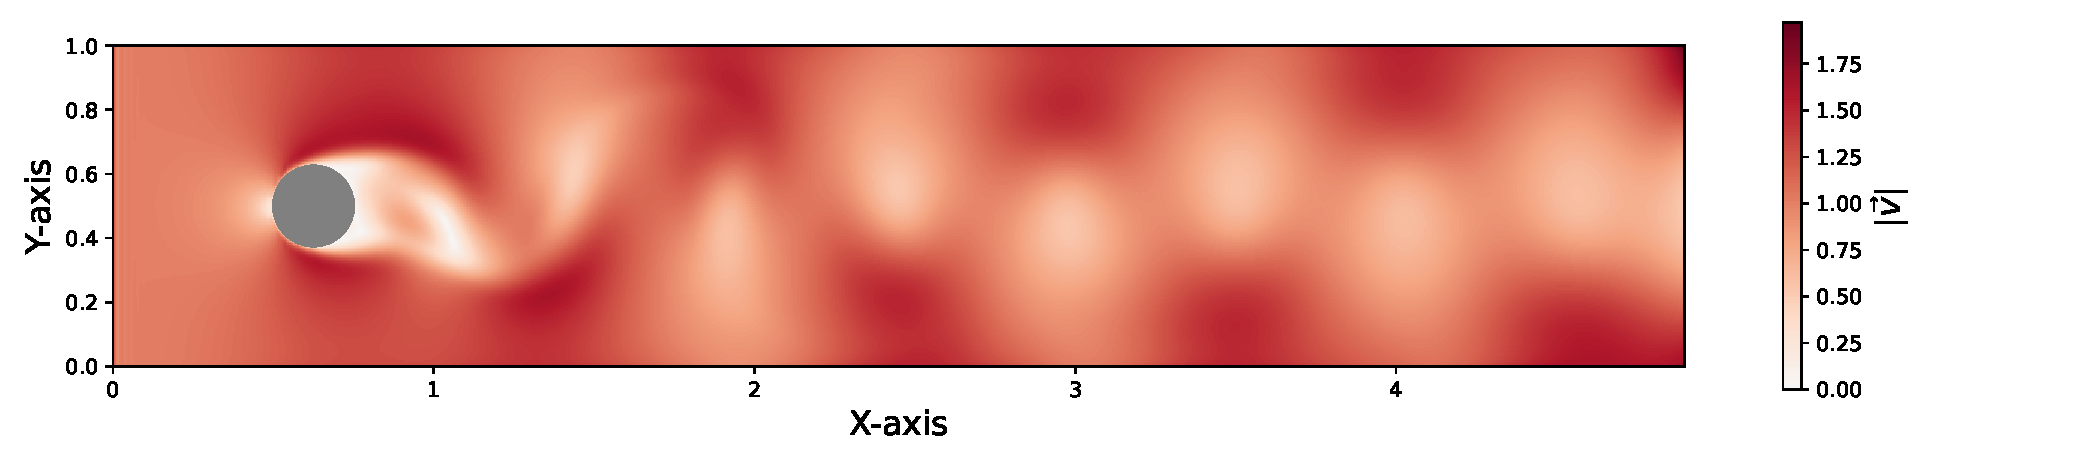
\includegraphics[width=\linewidth]{0_graphics/numeric/absV_25_sim.pdf}
        \caption{Magnitude of the velocity $\sqrt{u^2+v^2}$}
        \label{fig:abs_velocity_25}
    \end{subfigure}
    \vspace{1em} % Adjust space between subfigures as needed
    \hspace*{0.7cm}
    \begin{subfigure}[b]{\linewidth} % Adjust the width as needed
        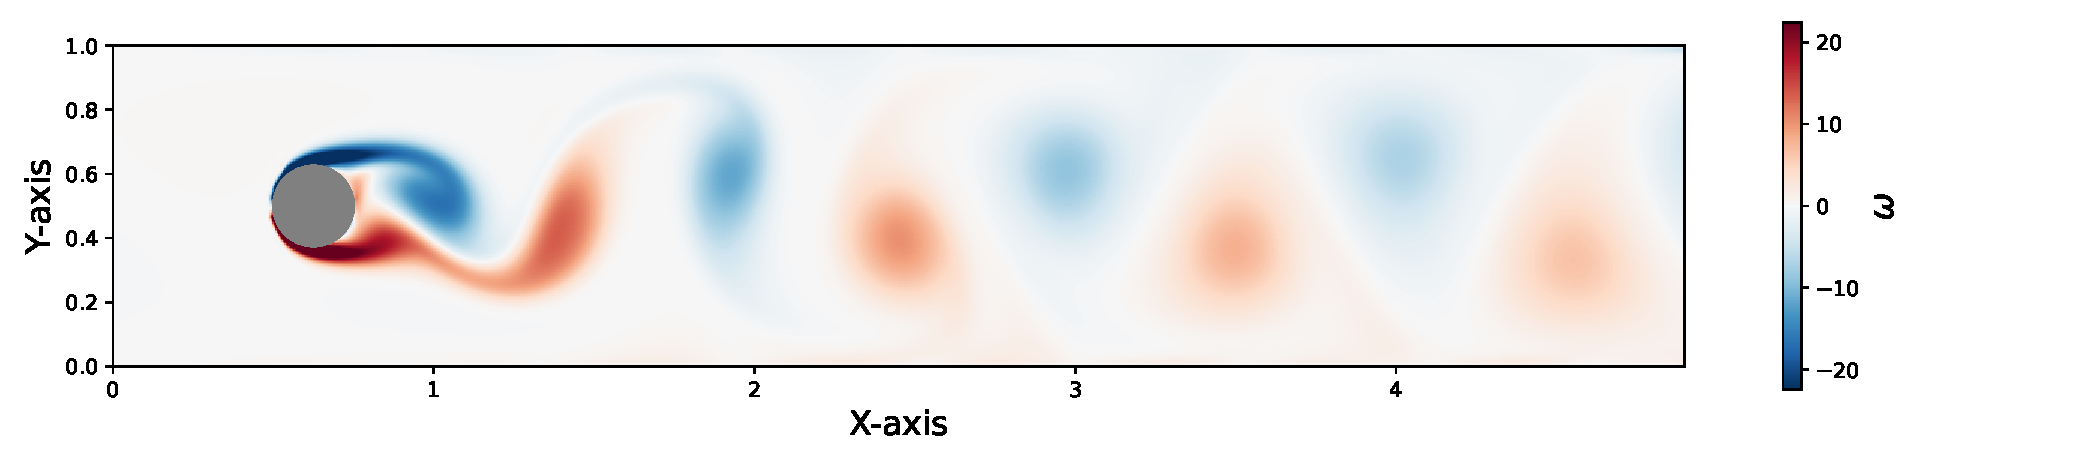
\includegraphics[width=\linewidth]{0_graphics/numeric/vor_25_sim.pdf} % Assuming a different file for vorticity
        \caption{Vorticity $\omega$.}
        \label{fig:vorticity_25}
    \end{subfigure}
    \vspace{-15pt}
    \caption{Flow dynamics around a circular obstacle in a fluid with Reynolds number $\Rey = 500$ at time $t=25$. The top image displays the magnitude of the velocity $\sqrt{u^2+v^2}$, and the bottom image focuses on the vorticity $\omega$.}
    \label{fig:first_karman}
\end{figure}
The time step is taken in an adaptative way, in order to ensure the CFL condition discussed in \cref{sec: diffScheme}. On the right side of the domain we place a circle with radius $r = 0.125$ as an object and at the start of the simulation the fluid inside the domain is at rest. Imposing the boundary conditions as presented in \cref{sec: posingProblem}, the fluid starts to move from the left side to the right side of the domain.
As the simulation progresses, the flow dynamics evolve to reveal the organized structure known as a von Kármán vortex street. In \cref{fig:first_karman}, we present the outcomes of this prolonged simulation, showcasing the magnitude of the velocity field and the vorticity $ \omega=\nabla \times \vf{u} = \frac{\partial v}{\partial x} - \frac{\partial u}{\partial y}$, to visualize the vortices. The vorticity measures the local rotation of the velocity field. In the figure we can observe the characteristic periodicity between red (counterclockwise rotating vortices) and blue (clockwise rotating vortices) vortices. In front of the body the flow seems to be laminar with an income velocity of approximately $u = 1$ (after normalization), which is consistent with our boundary conditions.



\subsection{Influence of Reynolds number}
% Analysis how high low reynoldsnumber influence the flow and the phenomenon Maybe there is a limit for our solver or there is a limit for the phenomenon 
The Reynolds number plays an important role in determining the flow characteristics around bodies in a fluid. It serves as a crucial indicator for the flow regime around bodies immersed in a fluid, significantly influencing the resulting flow patterns. In this section, we look at the same setup as before and vary the Reynolds number. The impact can be categorized in different regimes. In \cref{fig:influenceRey1} we plot the vorticity of the flow for different Reynolds numbers. 

\begin{figure}[!htb]
    \centering
    \hspace*{0.7cm}
    \begin{subfigure}[b]{\linewidth} % Adjust the width as needed
        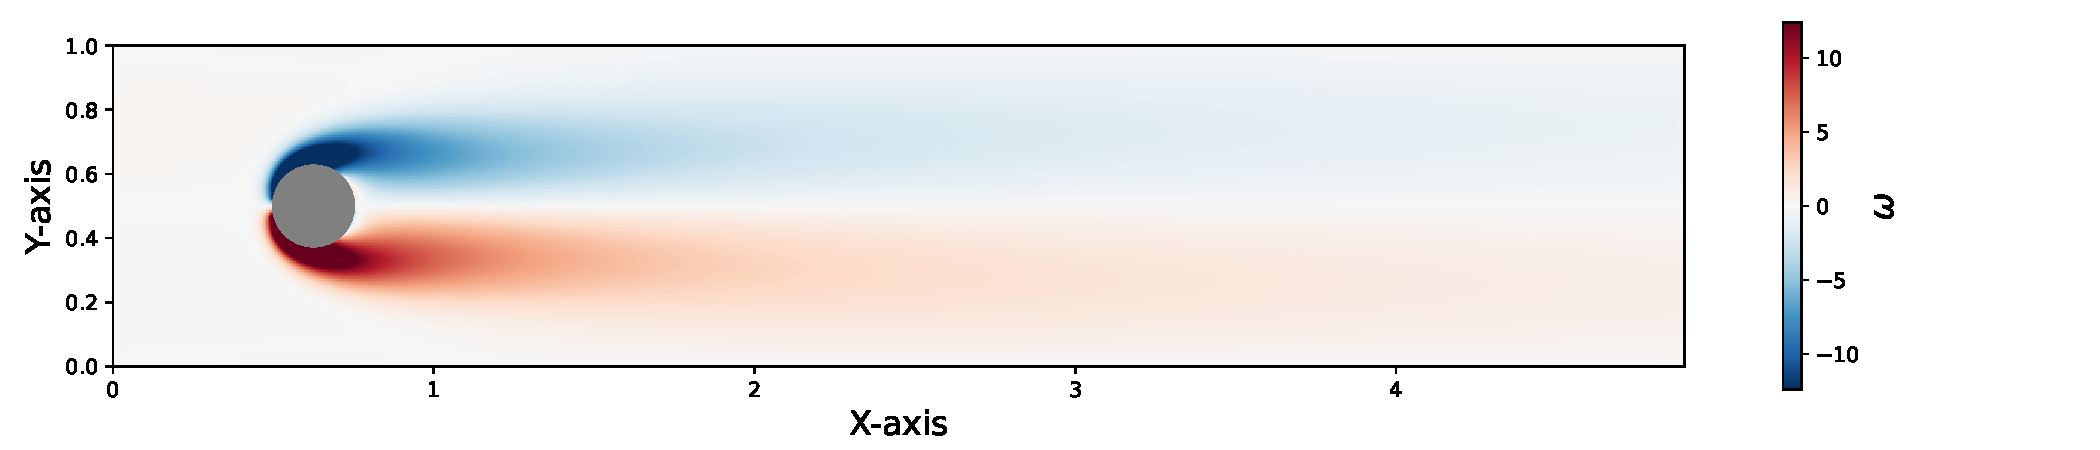
\includegraphics[width=\linewidth]{0_graphics/numeric/RE100_30_sim.pdf}
        \caption{Vorticity $\omega$ for $\Rey = 100$}
        \label{fig:RE100_vor_40}
    \end{subfigure}

    \hspace*{0.7cm}
    \begin{subfigure}[b]{\linewidth} % Adjust the width as needed
        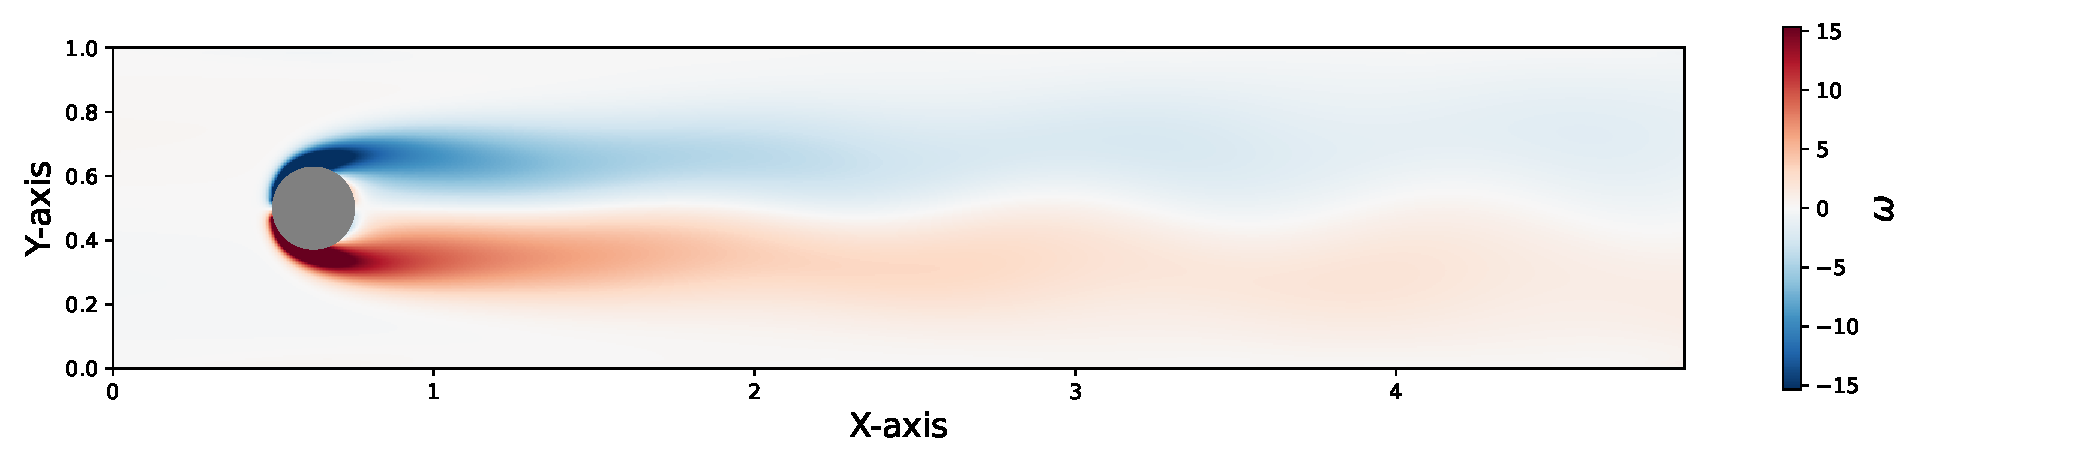
\includegraphics[width=\linewidth]{0_graphics/numeric/RE175_30_sim.pdf}
        \caption{Vorticity $\omega$ for $\Rey = 175$}
        \label{fig:RE175_vor_40}
    \end{subfigure}

        \hspace*{0.7cm}
    \begin{subfigure}[b]{\linewidth} % Adjust the width as needed
        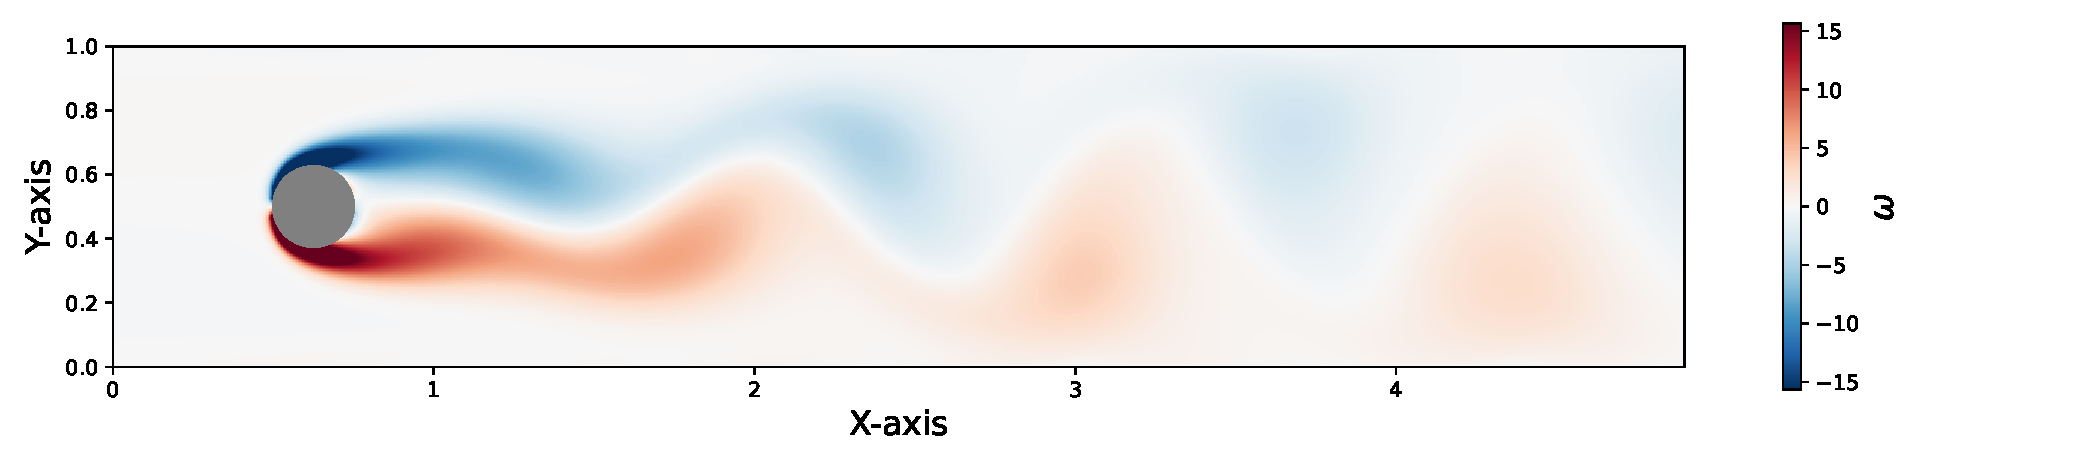
\includegraphics[width=\linewidth]{0_graphics/numeric/RE190_30_sim.pdf}
        \caption{Vorticity $\omega$ for $\Rey = 190$}
        \label{fig:RE190_vor_40}
    \end{subfigure}

        \hspace*{0.7cm}
    \begin{subfigure}[b]{\linewidth} % Adjust the width as needed
        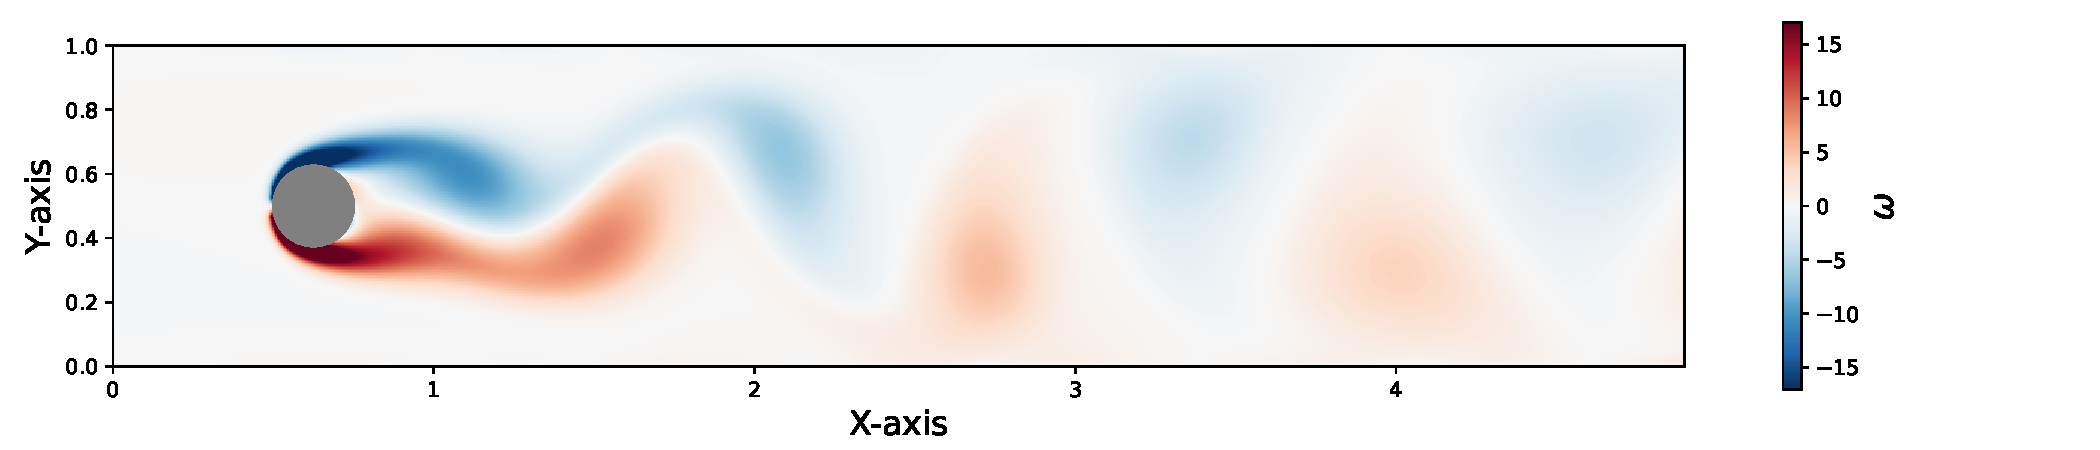
\includegraphics[width=\linewidth]{0_graphics/numeric/RE230_30_sim.pdf} 
        \caption{Vorticity $\omega$ for $\Rey = 230$}
        \label{fig:RE230_vor_40}
    \end{subfigure}

    \vspace{-5pt}
    \caption{Flow dynamics around a circular obstacle for fluid with different Reynolds numbers at time $t=30$.}
    \label{fig:influenceRey1}
\end{figure}

The impact of the Reynolds number is evident. For low Reynolds numbers ($\Rey \leq 150$) the flow stays laminar, and pattern formation is not observed. For $\Rey \approx 175$ the flow starts to be more complex. We don't observe vortices, but behind the body the vertical velocity periodically changes. Increasing the Reynolds number further we observe that the periodic perturbation become stronger ($\Rey = 190$), until finally vortices emerge ($\Rey \geq 230$).


\subsection{Influence of the object}
We this section we aim to demonstrate the impact of object geometry on the flow characteristics. To show that the geometry of objects immersed in a fluid significantly influences the flow patterns that develop around them, we look at a more advanced shape: an airfoil. This shape is not just designed to create lift for a plane, but also to ensure that the flow patterns are stable and manageable. This stability is essential for effective maneuverability during flight.

\begin{figure}[!htb]
    \centering
    \hspace*{0.7cm}
    \begin{subfigure}[b]{\linewidth} % Adjust the width as needed
        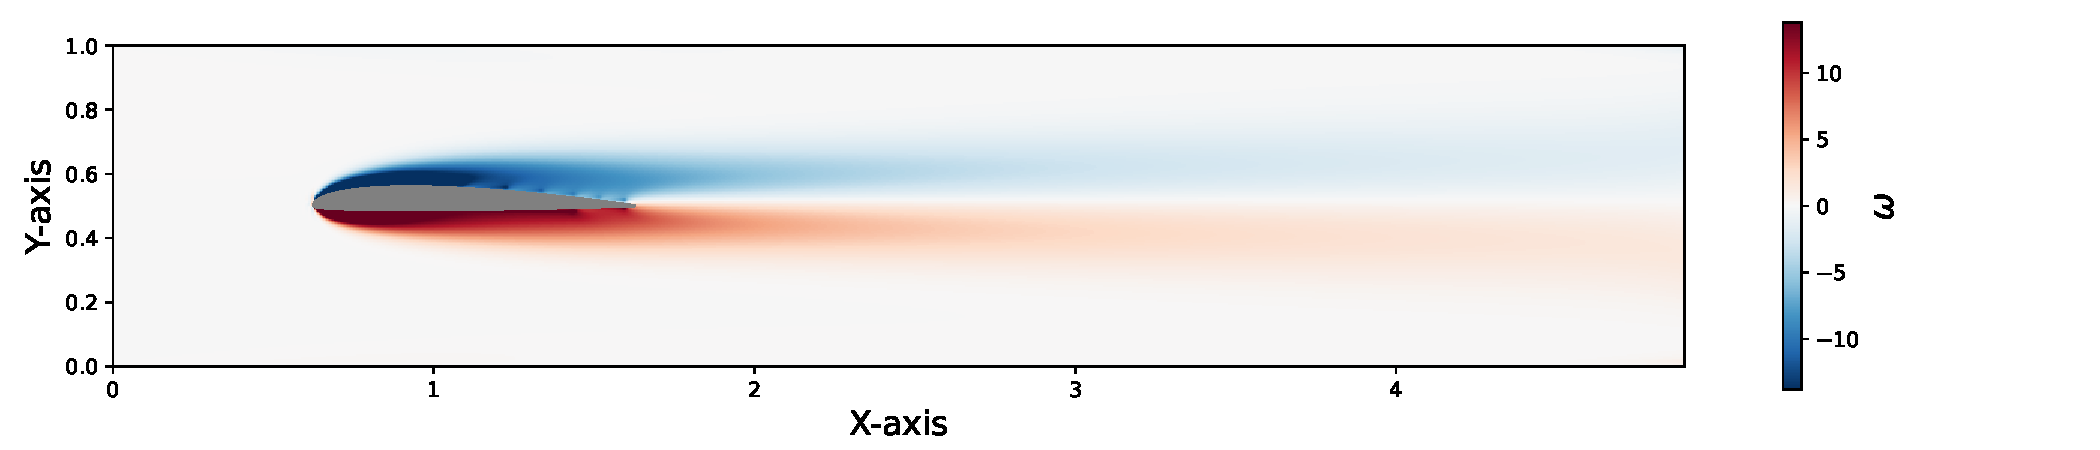
\includegraphics[width=\linewidth]{0_graphics/numeric/RE500_30_airfoil.pdf}
        \caption{Vorticity $\omega$ for $\Rey = 500$}
        \label{fig:RE500_airfoil}
    \end{subfigure}

    \hspace*{0.7cm}
    \begin{subfigure}[b]{\linewidth} % Adjust the width as needed
        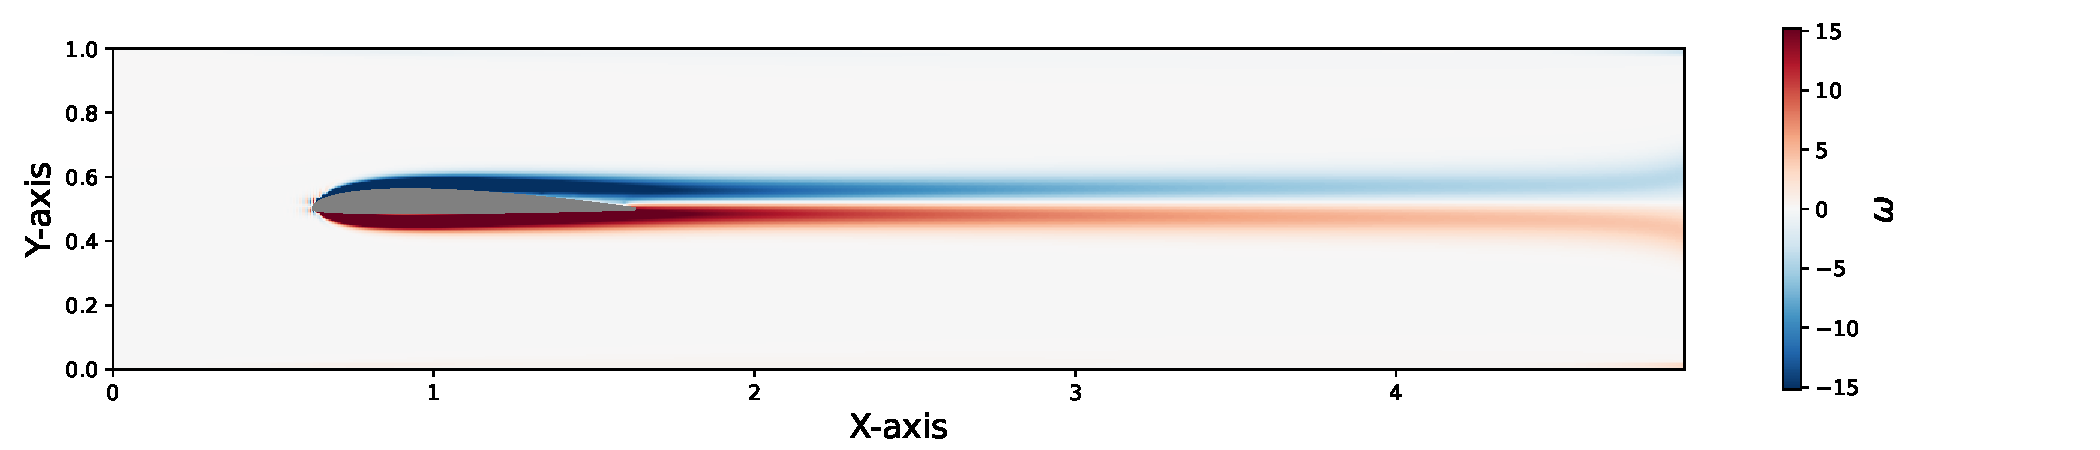
\includegraphics[width=\linewidth]{0_graphics/numeric/RE3500_30_airfoil.pdf}
        \caption{Vorticity $\omega$ for $\Rey = 3500$}
        \label{fig:RE3500_airfoil}
    \end{subfigure}

    \hspace*{0.7cm}
    \begin{subfigure}[b]{\linewidth} % Adjust the width as needed
        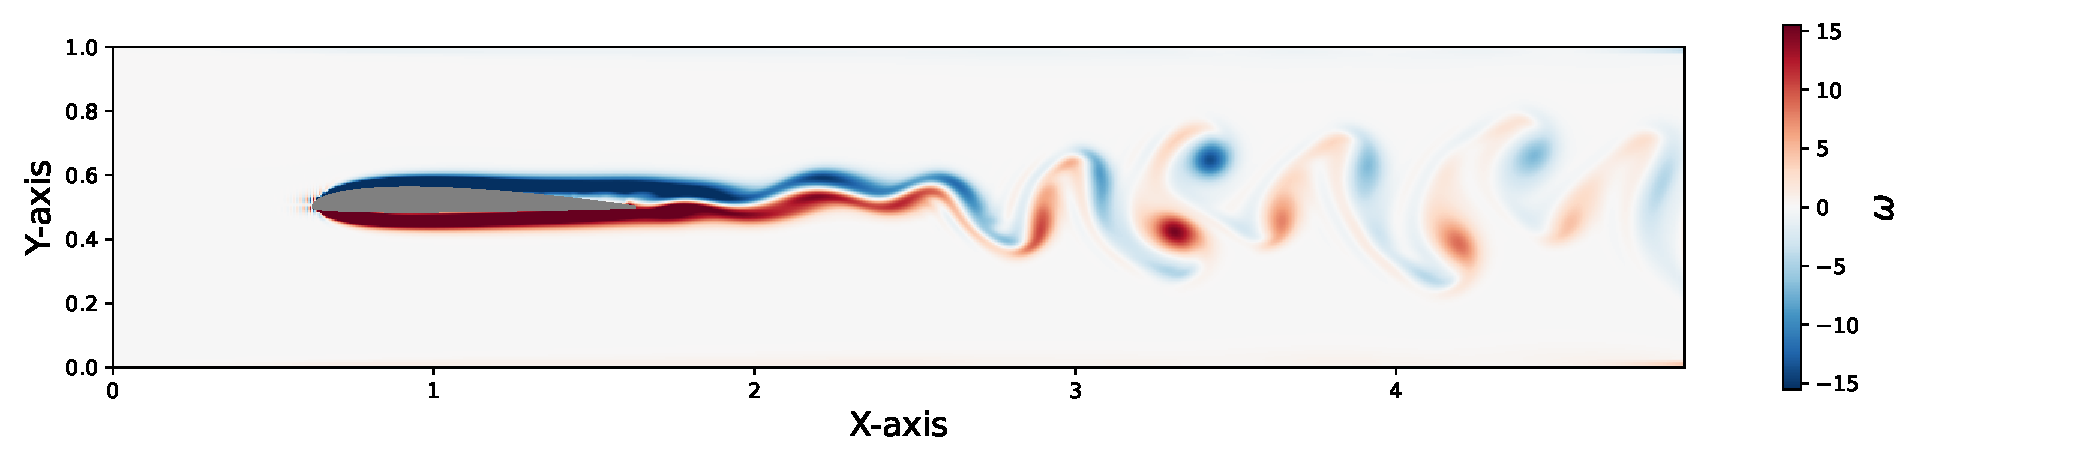
\includegraphics[width=\linewidth]{0_graphics/numeric/RE5500_30_airfoil.pdf}
        \caption{Vorticity $\omega$ for $\Rey = 5500$}
        \label{fig:RE5500_airfoil}
    \end{subfigure}

    \caption{Flow dynamics around an airfoil in a fluid with different Reynolds numbers at time $t=30$.}
    \label{fig:airfoil}
\end{figure}

In \cref{fig:RE500_airfoil}, we present our findings for the airfoil subjected to a Reynolds number $\Rey = 500$. In contrast with the observations made in \cref{fig:abs_velocity_25} for the circle, the flow surrounding the airfoil is remarkably devoid of vortices or significant flow perturbations. The elongated shape reduces the region in which the side eddies can interact and delays the onset of mixing to a position much farther behind the object. This difference demonstrates the influence of object geometry on flow dynamics. The streamlined shape of the airfoil leads to smoother flow, reducing the tendency for vortex formation.

It is important to note that comparing flows around bodies of dissimilar shapes at equivalent Reynolds numbers is inherently challenging. This challenge arises due to the variability in characteristic lengths and velocities, which fundamentally alters the flow's nature around each object. But even increasing the Reynolds number to $\Rey=3500$, does not lead to turbulences in the flow. As we can see in \cref{fig:RE3500_airfoil} the flow around the airfoil maintains a predominantly laminar characteristic, a testament to its aerodynamically efficient design. 

Only when we further increase the Reynolds number to $\Rey=5500$, the flow around the airfoil begins to exhibit clear signs of turbulence, marked by the formation of vortices. In \cref{fig:RE5500_airfoil} we plot the results and we can clearly see vortices arising behind the foil. The circle, with its inherent propensity to induce turbulence, resulted in flow conditions too chaotic for our solver to accurately simulate over extended durations. 

In the case of the airfoil we see that the influence of the shape on flow dynamics is very important. This underscores the significance of the complexity in designing aircraft that must operate effectively across a broad range of speeds. As a result, the design of wings is not only highly optimized but, in certain cases, incorporates the ability to change shape dynamically to adapt optimally to the aircraft's velocity.
% \newpage

\section{Conclusion}
% Desribe what we achieved (solver)
% What did we find out (Influence of viscosity and shape)
% Relevance of our findings, other interesting questions
In this report we numerically analysed the von Kármán vortex street. We successfully built a solver which leverages Chorin's method to simplify the integration step and breaks it down in smaller steps, which are easier to solve. The method then simplified to treating the advection with a second order Semi-Lagrangian scheme, the diffusion with a second order central difference scheme and the Poisson equation for the pressure with a 5-point stencil method. To achieve great flexibility for the possible shapes inside the domain, we impose the fluid at rest in the form of the shape. Basically, this corresponds to imposing a no-slip condition at the boundary of the shape.

In the second part of our approach we numerically investigated the emergent flow patterns around different objects. First, we exemplary showed the emergence of the von Kármán vortex street in case of a circle placed on the left side of the domain for fluid with intermediate Reynolds numbers. As expected we observe the alternating vortices behind the body. We identified a critical Reynolds number which indicates the dynamics of the flow. For smaller Reynolds numbers the flow is laminar and no vortices emerge. For higher numbers periodic formations emerge, which finally lead to mixing and vortices shredding. Finally, we demonstrated the impact of the shape on the flow. By looking at an airfoil we showed that with intelligent design of the shape the dynamics of the flow can be greatly influenced. With this new shape only with much higher Reynolds numbers we observed vortex shredding and thereby showcased the importance of fluid- and aero-dynamic favorable design. Especially for planes, ships or turbines the shape has a great impact on performance and efficiency, among other essential performance metrics.\label{sec: conclusion}
\newpage

% ###################################################################
% ######## References
% ###################################################################

%\bibliographystyle{unsrt}
%\bibliography{refs}
\phantomsection
\addcontentsline{toc}{section}{References}
\printbibliography

% \newpage
\end{document}

